\documentclass[a4paper,showframe,11pt]{report}\usepackage[]{graphicx}\usepackage[]{color}
%% maxwidth is the original width if it is less than linewidth
%% otherwise use linewidth (to make sure the graphics do not exceed the margin)
\makeatletter
\def\maxwidth{ %
  \ifdim\Gin@nat@width>\linewidth
    \linewidth
  \else
    \Gin@nat@width
  \fi
}
\makeatother

\definecolor{fgcolor}{rgb}{0.196, 0.196, 0.196}
\newcommand{\hlnum}[1]{\textcolor[rgb]{0.063,0.58,0.627}{#1}}%
\newcommand{\hlstr}[1]{\textcolor[rgb]{0.063,0.58,0.627}{#1}}%
\newcommand{\hlcom}[1]{\textcolor[rgb]{0.588,0.588,0.588}{#1}}%
\newcommand{\hlopt}[1]{\textcolor[rgb]{0.196,0.196,0.196}{#1}}%
\newcommand{\hlstd}[1]{\textcolor[rgb]{0.196,0.196,0.196}{#1}}%
\newcommand{\hlkwa}[1]{\textcolor[rgb]{0.231,0.416,0.784}{#1}}%
\newcommand{\hlkwb}[1]{\textcolor[rgb]{0.627,0,0.314}{#1}}%
\newcommand{\hlkwc}[1]{\textcolor[rgb]{0,0.631,0.314}{#1}}%
\newcommand{\hlkwd}[1]{\textcolor[rgb]{0.78,0.227,0.412}{#1}}%
\let\hlipl\hlkwb

\usepackage{framed}
\makeatletter
\newenvironment{kframe}{%
 \def\at@end@of@kframe{}%
 \ifinner\ifhmode%
  \def\at@end@of@kframe{\end{minipage}}%
  \begin{minipage}{\columnwidth}%
 \fi\fi%
 \def\FrameCommand##1{\hskip\@totalleftmargin \hskip-\fboxsep
 \colorbox{shadecolor}{##1}\hskip-\fboxsep
     % There is no \\@totalrightmargin, so:
     \hskip-\linewidth \hskip-\@totalleftmargin \hskip\columnwidth}%
 \MakeFramed {\advance\hsize-\width
   \@totalleftmargin\z@ \linewidth\hsize
   \@setminipage}}%
 {\par\unskip\endMakeFramed%
 \at@end@of@kframe}
\makeatother

\definecolor{shadecolor}{rgb}{.97, .97, .97}
\definecolor{messagecolor}{rgb}{0, 0, 0}
\definecolor{warningcolor}{rgb}{1, 0, 1}
\definecolor{errorcolor}{rgb}{1, 0, 0}
\newenvironment{knitrout}{}{} % an empty environment to be redefined in TeX

\usepackage{alltt}
\usepackage{standalone}
\standalonetrue
\ifstandalone
  \usepackage{../../haziq_thesis}
  \usepackage{../../haziq_maths}
  \usepackage{../../haziq_glossary}
  \addbibresource{../../bib/haziq.bib}
  \externaldocument{../01/.texpadtmp/introduction}
\fi







\IfFileExists{upquote.sty}{\usepackage{upquote}}{}
\begin{document}

\hltodo{cite Hastie Tibshirani elements of statistical learning}.
We illustrate multiclass classification using I-priors on a speech recognition data set\footnotemark with $m = 11$ classes to be predicted from digitized low pass filtered signals generated from voice recordings.
Each class corresponds to a vowel sound made when pronouncing a specific word.
The words that make up the vowel sounds are shown in Table \ref{tab:vowel}. Each word was uttered once by multiple speakers, and the data are split into a training and a test set.
Four males and four female speakers contributed to the training set, while four male and three female speakers contributed to the test set.
The recordings were manipulated using speech processing techniques, such that each speaker yielded six frames of speech from the eleven vowels, each with a corresponding 10-dimensional numerical input vector (the predictors).
This means that the size of the training set is 528, while 462 data points are available for testing the predictive performance of the models.
This data set is also known as Deterding's vowel recognition data (after the original collector, cite) or the Connectionist Bench data.
Machine learning methods such as neural networks and nearest neighbour methods were analysed by Robinson (cite).

\footnotetext{Data is publicaly available from the UCI Machine Learning Repository, URL: \url{https://archive.ics.uci.edu/ml/datasets/Connectionist+Bench+(Vowel+Recognition+-+Deterding+Data)}.}

\begin{table}[]
\centering
\caption{The eleven words that make up the classes of vowels.}
\label{tab:vowel}
\begin{tabular}{llllllllll}
\toprule
Class & Label          & Vowel & Word &  && Class & Label          & Vowel & Word  \\
\midrule
1     & \texttt{hid} & \dsil{iː}    & heed &&  & 7     & \texttt{hOd} & \dsil{ɒ}    & hod   \\
2     & \texttt{hId} & \dsil{ɪ}     & hid  &&  & 8     & \texttt{hod} & \dsil{ɔː}   & hoard \\
3     & \texttt{hEd} & \dsil{ɛ}     & head &&  & 9     & \texttt{hUd} & \dsil{ʊ}    & hood  \\
4     & \texttt{hAd} & \dsil{a}     & had  &&  & 10    & \texttt{hud} & \dsil{uː}   & who'd \\
5     & \texttt{hYd} & \dsil{ʌ}     & hud  &&  & 11    & \texttt{hed} & \dsil{əː}   & heard \\
6     & \texttt{had} & \dsil{ɑː}    & hard &&  &       &              &             &       \\
\bottomrule
\end{tabular}
\end{table}

We will fit the data using an I-probit model with the canonical linear kernel and also the fBm-0.5 kernel.
We assume $m = 11$ distinct I-priors corresponding to the latent variables in each class, thus there are 11 unique intercepts and 11 RKHS scale parameters to estimate in each model.
Each model took roughly 6 seconds per iteration to complete.
The canonical kernel model took a long time to converge, with each variational EM iteration improving the lower bound only slighly each time.
In contrast, the fBm-0.5 model was quicker to converge, and this is something that we noticed happening for most other data sets as well.
Multiple restarts from different random seeds were conducted, and we found that they all converged to a similar lower bound value.
This alleviates any worry that the model might have converged to different multiple local optima.

\begin{knitrout}
\definecolor{shadecolor}{rgb}{1, 1, 1}\color{fgcolor}\begin{figure}[h]

{\centering \subfloat[Canonical kernel\label{fig:vowel.confusion.matrix1}]{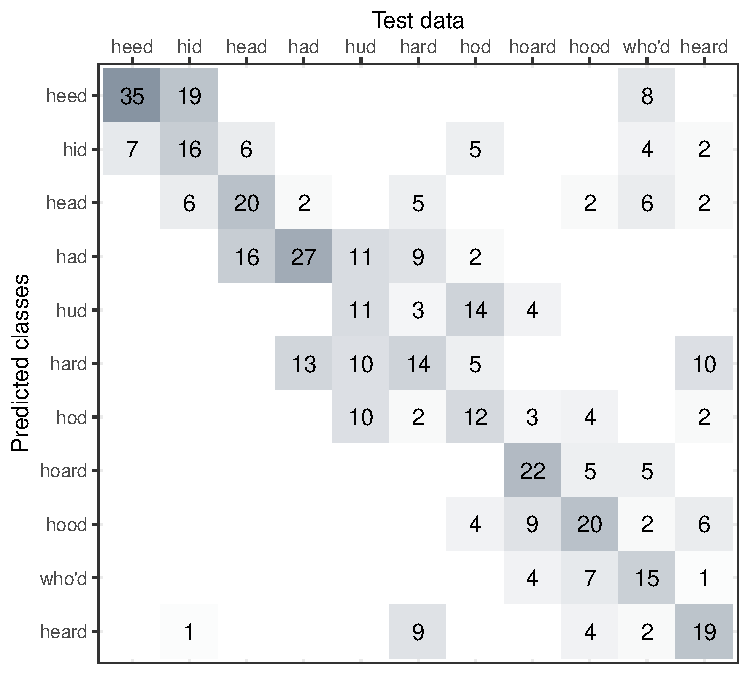
\includegraphics[width=0.485\linewidth]{figure/vowel_confusion_matrix-1} }
\subfloat[fBm-0.5 kernel\label{fig:vowel.confusion.matrix2}]{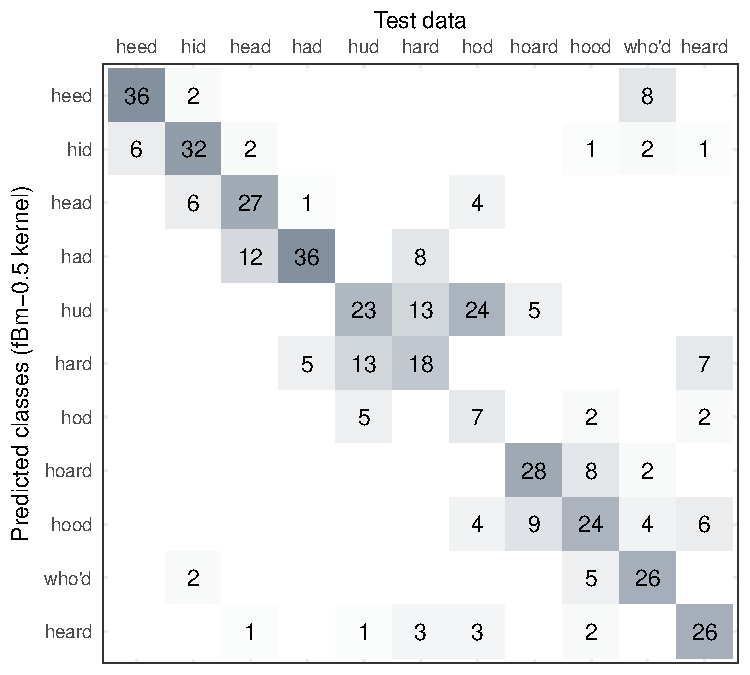
\includegraphics[width=0.485\linewidth]{figure/vowel_confusion_matrix-2} }

}

\caption[Confusion matrices for the vowel classification problem in which predicted values were obtained from the I-probit models]{Confusion matrices for the vowel classification problem in which predicted values were obtained from the I-probit models. The maximum value for any one cell is 42. Blank cells indicate nil values.}\label{fig:vowel.confusion.matrix}
\end{figure}


\end{knitrout}

A good way to visualise the performance of model predictions is through a confusion matrix, as shown in Figure \ref{fig:vowel.confusion.matrix}. The numbers in each row indicate the instances of a predicted class, while the numbers in the column indicate instances of the actual classes. Nil values are indicated by blank cells. A quick glance of the plots seem to favour the fBm-0.5 kernel as having better predictions. There are a lot more misclassifications when using the canonical kernel. Under the fBm-0.5 model, the model makes understandable mistakes - confusing very similar words, especially `hod' and `hud'.

Comparisons to other methods that had been used to analyse this data set is given in Table \ref{tab:vowel.tab}.
In particular, the I-probit model is compared against 1) linear regression; 2) logistic linear regression; 3) linear and quadratic discriminant analysis; 4) decision trees; 5) neural networks; 6) $k$-nearest neighbours; and 7) flexible discriminant analysis.
All of these methods are described in further detail in cite{Hastie Tibshirani}.
The I-probit model using the fBm-0.5 kernel offers one of the best out-of-sample classification error rates (38.7\%) of all the methods compared.
The linear I-probit model is seen to be comparable to logistic regression, linear and quadratic discrimant analysis, and also decision trees.
It also provides significant improvement over multiple linear regression.

\begin{knitrout}
\definecolor{shadecolor}{rgb}{1, 1, 1}\color{fgcolor}\begin{table}

\caption{\label{tab:vowel.tab}Results of various classification methods for the vowel data set.}
\centering
\begin{tabular}[t]{lrr}
\toprule
\multicolumn{1}{c}{ } & \multicolumn{2}{c}{Error rates} \\
\cmidrule(l{2pt}r{2pt}){2-3}
Method & Training & Test\\
\midrule
Linear regression & 48 & 67\\
Logistic regression & 22 & 51\\
Linear discriminant analysis & 32 & 56\\
Quadratic discriminant analysis & 1 & 53\\
\addlinespace
Decision trees & 5 & 54\\
Neural networks &  & 45\\
k-Nearest neighbours &  & 44\\
FDA/BRUTO & 6 & 44\\
FDA/MARS & 13 & 39\\
\addlinespace
I-probit (fBm-0.5) & 22 & 39\\
I-probit (linear) & 28 & 54\\
\bottomrule
\end{tabular}
\end{table}


\end{knitrout}

\end{document}


